\section{Background and Overview} \label{sec:background} 
\begin{figure*}[t]
\begin{center}
\begin{tabular}{ccc}
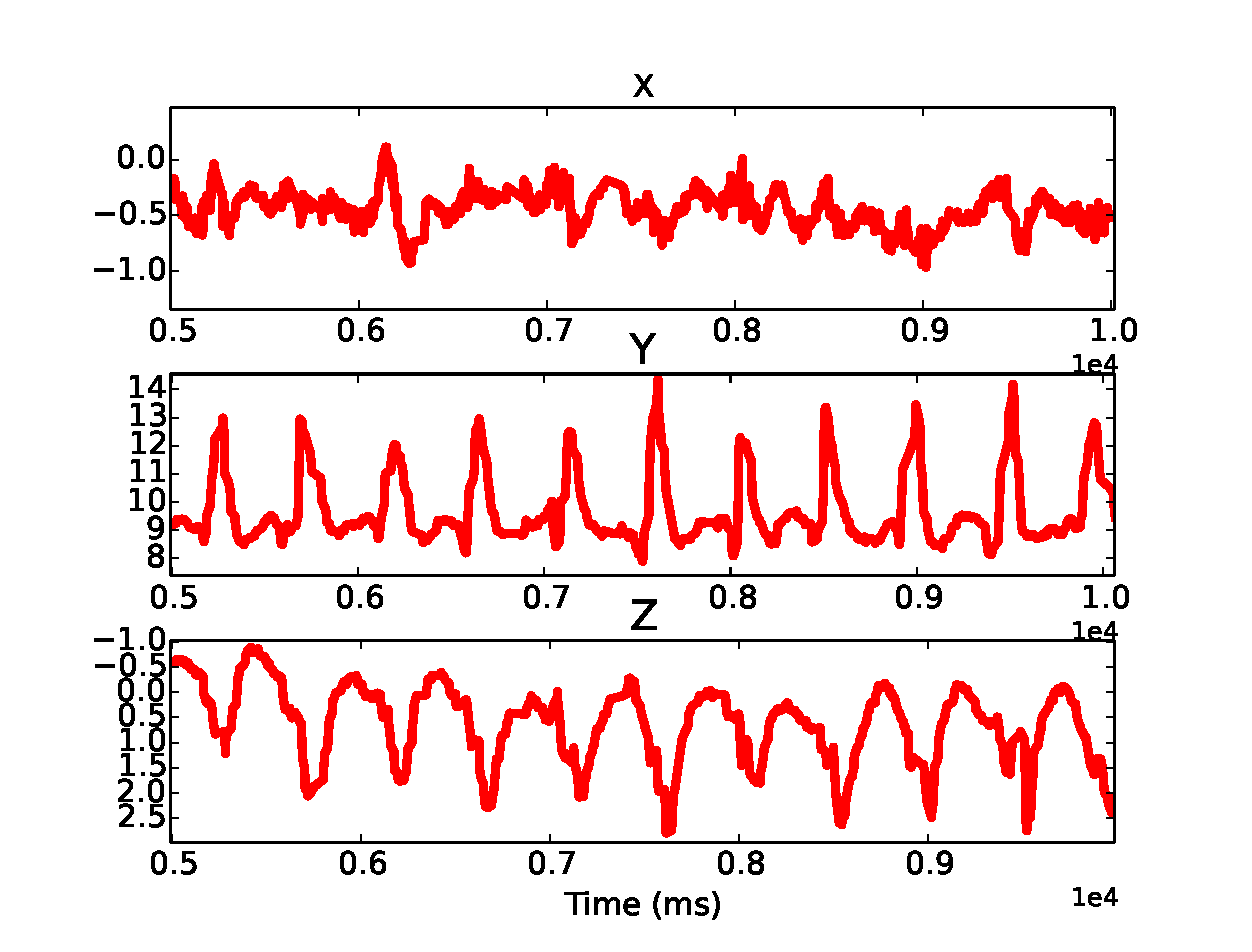
\includegraphics [width=.33\linewidth]{../mobisys_paper/fig/raw_sub1.eps}&
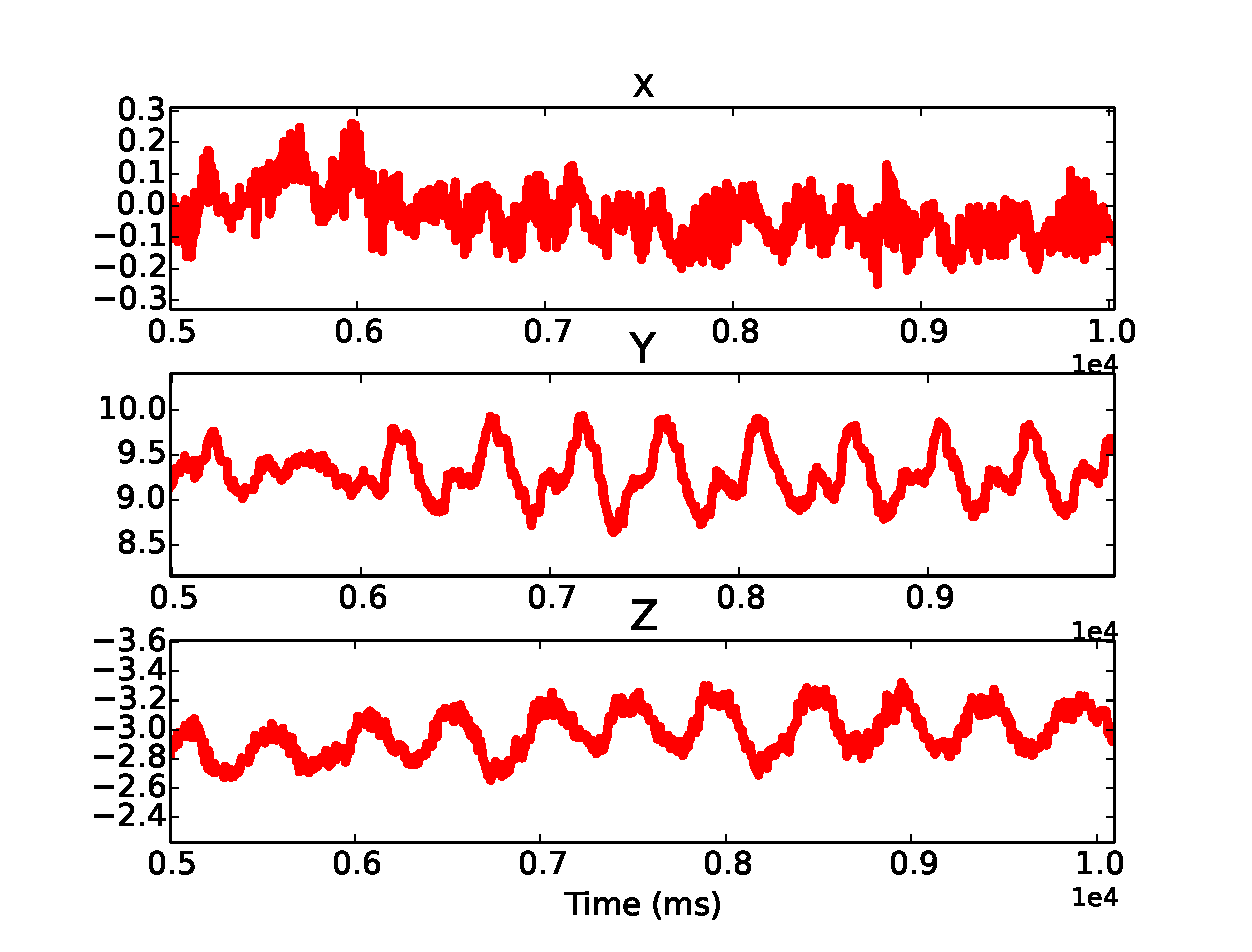
\includegraphics [width=.33\linewidth]{../mobisys_paper/fig/raw_sub8.eps}&
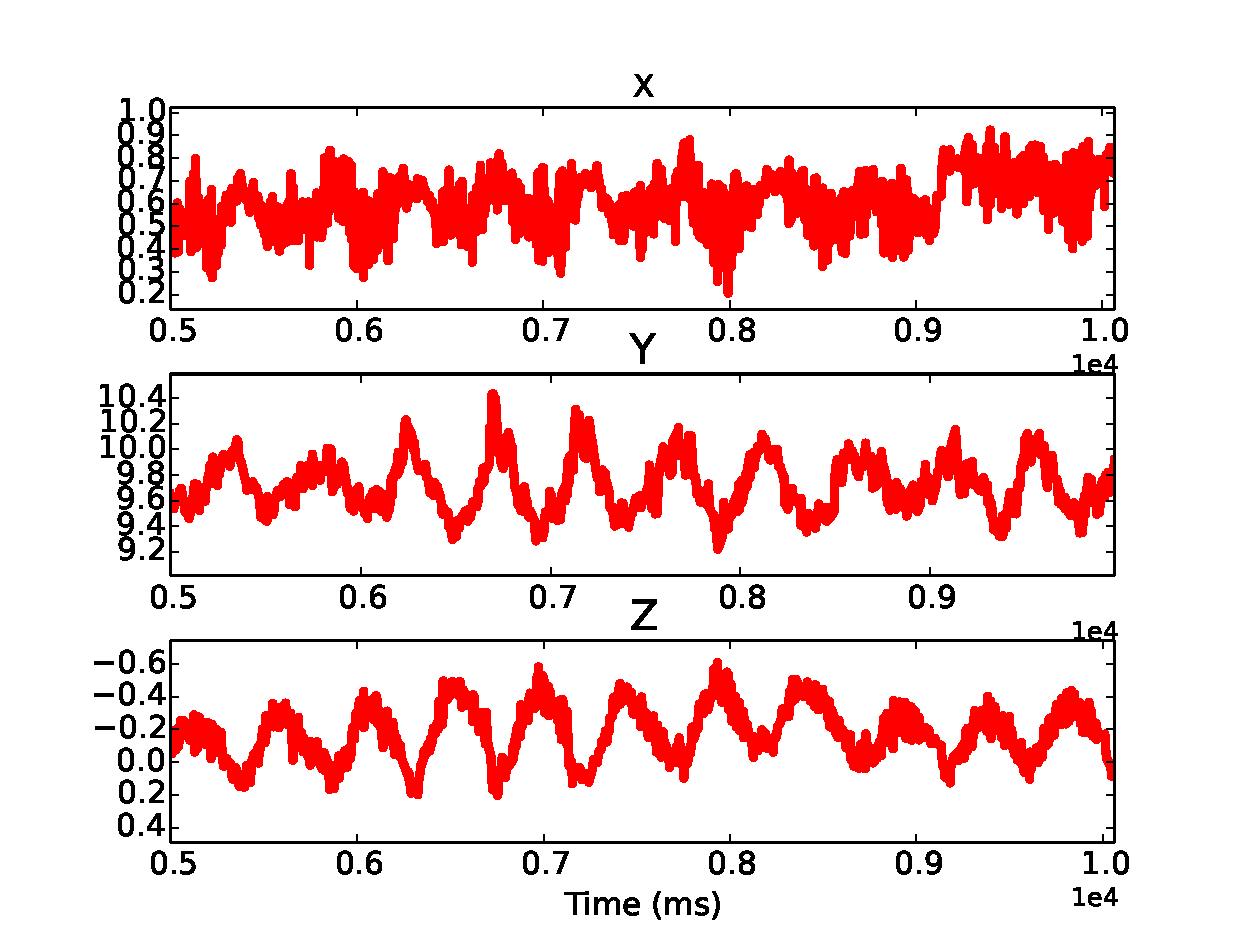
\includegraphics [width=.33\linewidth]{../mobisys_paper/fig/raw_sub3.eps}\\
(a) User 1& (b) User 2 & (c) User 3 \\
\end{tabular}

\begin{tabular}{cc}
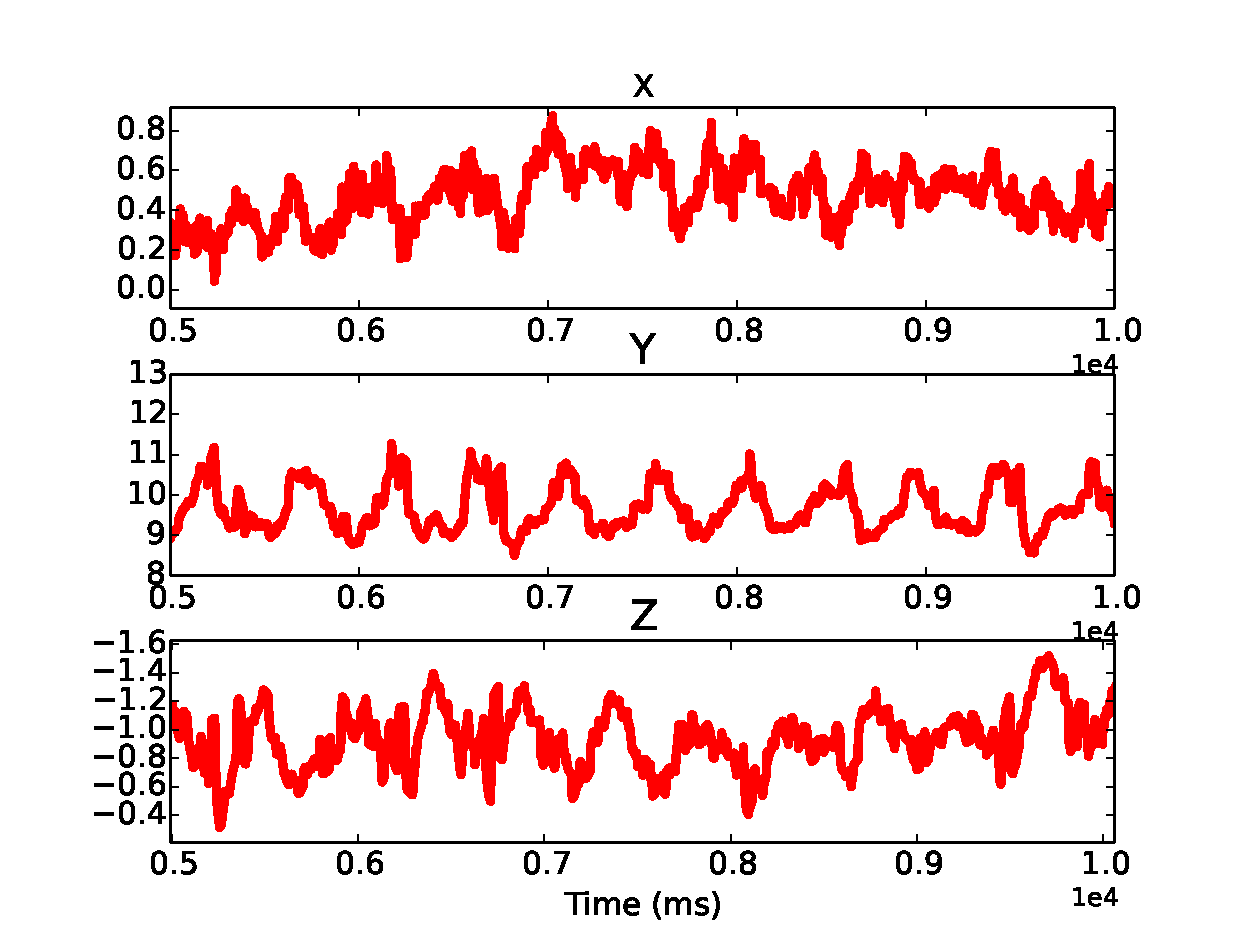
\includegraphics [width=.33\linewidth]{../mobisys_paper/fig/raw_sub4.eps}&
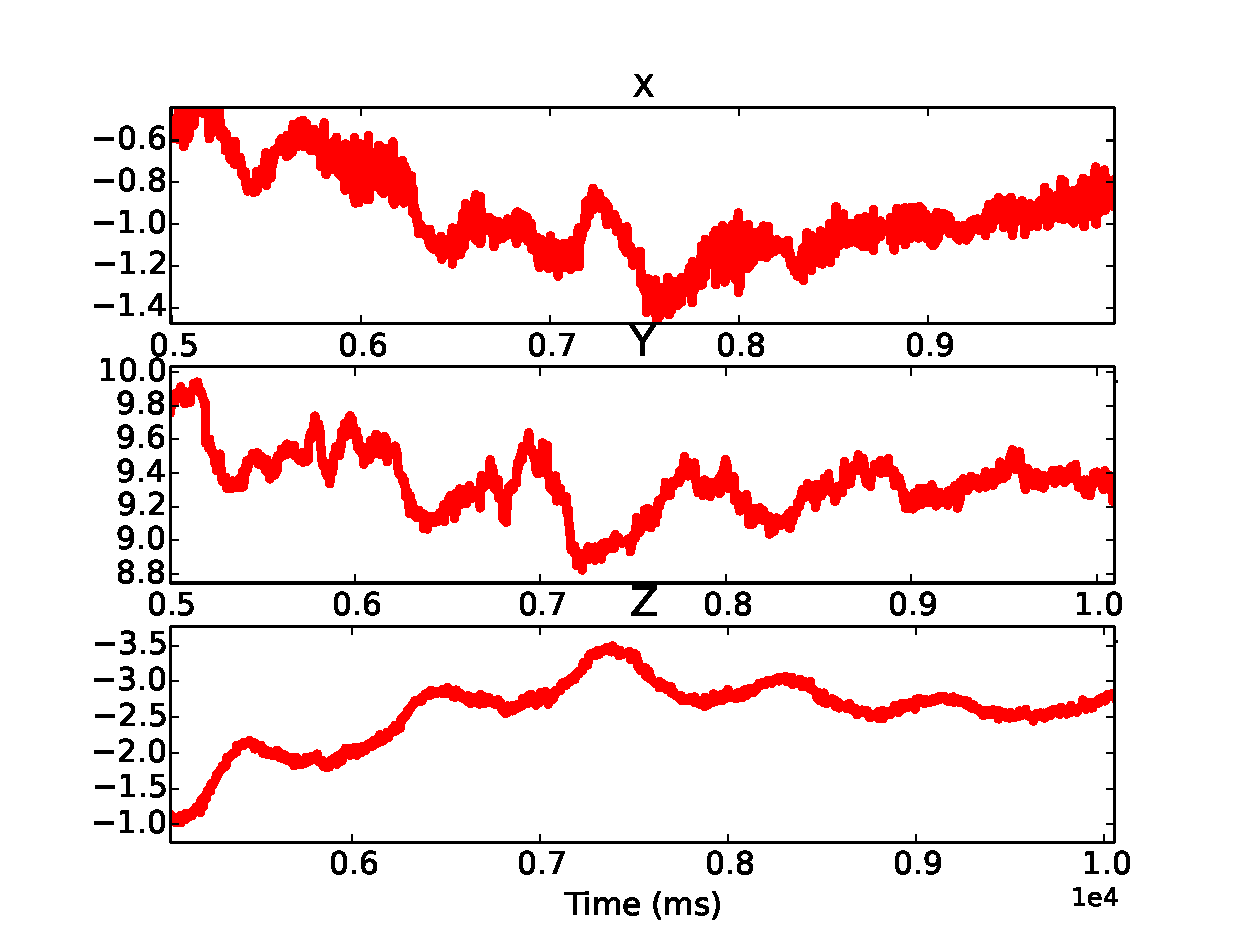
\includegraphics [width=.33\linewidth]{../mobisys_paper/fig/raw_sub5.eps}\\
(d) User 4& (e) User 5 \\
\end{tabular}
\end{center}
\caption{\label{fig:raw} These plots show the raw accelerometer data in the
time domain for five different users when they move their head in response to
a music track wearing the same Google glass. The plots
indicate that different users' head movement patterns appear distinctive from
each other. The five users wore a Google Glass (in turns) and listened to a
10 second audio snapshot of a pop song.}
\end{figure*}

\subsection{Background on Behavioral Biometrics}
%Authentication mechanisms for a wearable device can broadly be divided into two
%categories: (i) {\em Direct} authentication, where the users can directly
%authenticate themselves to their wearable device using the input/output
%interface and/or using signatures generated from the sensors available on the
%device, and (ii) {\em Indirect} authentication, where a secondary device --
%typically the user's smartphone -- is used as a medium for authentication.
%Today's commercially available wearable devices predominantly use the latter
%approach where users login to their wearable devices through their smartphone
%-- using a PIN or an email account.


%Unlike the indirect approaches, that require a wearable device is registered to
%and connected (wireless) to a smartphone, direct
%mechanisms can leverage the built-in interfaces and sensors on the
%wearable device.
Considering the fact that wearable devices relate significantly to ``what we wear" on the
human body, biometrics can play a key role for direct authentication to wearable
devices. Biometrics allow a system to identify a user based upon ``who you
are" (i.e., her physiology) instead of ``what you
have'' (i.e., ID cards) or `` what you remember'' (i.e.,
passwords)~\cite{jain2004introduction,o2003comparing,yampolskiy2007motor}.
Physiological biometrics such as DNA, ear shape, face, fingerprint,
hand/finger geometry,
iris, odor, palm-print, retinal scan, and voice, have been very effective and
widely used in many prototype and commercial authentication systems~\cite{wu1997measure,yan2007biometric,zhao1998discriminant,hong1998fingerprint,wildes1997iris,
yan2007biometric,baldisserra2005fake,hill2002retina,markowitz2000voice,reynolds2000speaker,bowyer2006survey,biddle2012graphical,sherman2014user,jain1997identity}.
In addition, body shape such as body height, width, and body-part proportions
can also be used as biometric cues to identify different
people~\cite{collins2002silhouette}. Even ``soft'' characteristics such as
body weight and fat percentage have been considered as secondary biometrics
for authentication purposes~\cite{ailisto2006soft}.

However, biometrics are
not prominently used in wearable devices commercially available today, though
there have been specific point commercial designs (e.g., Nymi~\cite{nymi}). This can be attributed to the
fact that biometrics would require the specific hardware/sensor available on
the wearable device. Also the overheads for physiological biometrics in
wearable devices can be high, in both, cost for hardware as well as
integration and computing.

Another approach to direct authentication is using behavioral biometrics
where unique signatures from human behavior (subconscious
or in response to external stimulus) provide cues for differentiating and
authenticating users. For example, it has been shown that gait (e.g.,
stride length, the
amount of arm swing) when the user is walking or
running is a reliable identification cue, and irrespective of the
environment~\cite{stevenage1999visual}. Okumura et.al.~\cite{okumura2006study}
have shown that the human arm swing patterns can be used to create signatures
to authenticate to their cell-phones. Monrose
et.al.~\cite{monrose2000keystroke} show that keystroke rhythms, when
users type on the keyboard, that include typing dynamics such as how
long is a keystroke, how far is between consecutive strokes, and how is the
pressure exerted on each key, can be used as a biometric to authenticate
users. Similarly, mouse usage dynamics~\cite{jorgensen2011mouse} and touchpad
touching dynamics~\cite{bo2013silentsense,de2012touch} have also been shown to
serve as potential biometrics.

In comparison to other means of authentication, behavioral biometric authentication can offer a more convenient (than physiological biometrics),
and more secure (than indirect authentication) solution for wearable device
authentication. With the increasing off-the-shelf availability and (almost) unlimited access to the motion sensors on the wearables, it
has become possible to generate and/or infer unique behavioral signatures
specific to users. We use these rationale as a motivation for our proposed
design of a behavioral biometric based authentication that generates unique
signatures from user's body movements. We design an authentication system, dubbed {\em Headbanger}, for wearable
devices by monitoring user's body-movement patterns (e.g., head movements, arm movements, and hand movements) in response to an
external music stimulus. Here, we do not limit body movements to pre-defined templates; rather, the user chooses \emph{free-style} movement she feels the most natural to do.
%\vspace{4pt}{\bf Head-movements as a behavioral biometric.}

\subsection{Body Movement as a Behavioral Biometric}
\label{subsec:headmovements}

%As such, authenticating a user involves comparing her sensor
%readings with the pre-recorded glass owner's sensor readings.
%Our design assumes that there is only one owner per glass, and we can easily
%extend our scheme to handle the cases with multiple owners.
%Figure~\ref{fig:sysarch} presents the system architecture of the \systemname,
%and in the following section, we will discuss each component of this design
%in more detail.

According to~\cite{jain2004introduction}, a human characteristic can be
considered as biometric as long as it is \emph{universal}, \emph{distinctive},
\emph{repeatable}, and \emph{collectible}. With the advancements in
wearable computer designs it is becoming easier for collecting body movement
patterns using the built-in sensors (e.g., accelerometer sensor, gyroscope sensor, motion sensor, etc). Such sensors are
available on most wearable devices available today, thus
making body movements that are both \emph{universal} and {\em collectible}.

In this proposal, we will show that free-style natural body movements are \emph{distinctive} and \emph{repeatable}, especially when combined with external stimuli such as music. In~\systemname, music plays a crucial role in stimulating body movements such that the resulting movement pattern is natural to the user (more distinctive) and easier to remember (more repeatable). It has been shown~\cite{zentner2010rhythmic} that most people move
their body as a natural response to external rhythmic stimuli such as music;
even at a very early age, infants respond to music and their movements speed
up with the increasing rhythm speed. Most adults naturally
perform head movements or hand movements when listening to a fast beat audio track.  When combined with external rhythmic stimuli, we believe body movements become more distinctive -- not only a person's movement pattern is unique, but her response to rhythmic stimuli is also unique. In this way, the resulting authentication system will be more dependable.

Before we go ahead and design our system, we first conducted a preliminary analysis of the accelerometer signals from five Google glass
users' head movements, and show the raw signals in Figure~\ref{fig:raw} (a)-(e). A quick glance at the raw signals reveals that these users
{\em repeatedly} showed unique and {\em distinctive} head-movement patterns, when listening to the same music beats on the head-worn device. Motivated by this observation we hypothesize that \emph{body movements can be a good behavioral biometric characteristic to authenticate
users to their smart wearable device}.
%We next formally present the design of our system that
%utilizes head-movement patterns as behavioral biometric signature

\vspace{4pt}\textbf{Example Body Movement Patterns:} Depending upon the wearable device to be authenticated, we can focus on the movements of different body positions. For example, head-mounted devices such as smart glasses can easily capture a user's head movement or eye lid movements; wrist-mounted devices such as smart watches can easily capture a user's arm/hand movements; shoe-based smart devices can easily capture a user's gait; smart rings can easily capture a user's finger/palm movements.

To facilitate natural and repeatable body movements, we can play short, fast-tempo music tracks on the wearable devices, and measure the resulting body movements using built-in sensors such as accelerometer sensor, gyroscope sensor, infrared sensor, etc.



\vspace{4pt}\textbf{Earlier Work on Body Movement Based Activity Detection and Authentication:} There have been a few point solutions that used body gesture/movements (captured by sensors such as accelerometers and gyroscope) for activity detection or authentication purposes. For example, Harwin et al.~\cite{harwin1990analysis} used head gestures (e.g., combining pointing and movements) for human computer interaction. Eye blinking pattern was looked at in~\cite{westeyn2004recognizing} as a unique feature for authentication. Ishimaru et al.~\cite{ishimaru2014blink} proposed to combine the eye blinking frequency from the infrared proximity sensor and head motions from accelerometer sensor on Google Glass to recognize activities (e.g., reading, talking, watching TV, math problem solving, etc).
Accelerometers have also been used for other parts of body movements for gait analysis, motion detection or user identification, such as waist~\cite{ailisto2005identifying}, pocket~\cite{gafurov2007gait}, arm~\cite{okumura2006study,gafurov2008arm}, leg~\cite{gafurov2006biometric,karantonis2006implementation,mantyjarvi2005identifying,derawi2010unobtrusive} and ankle~\cite{gafurov2011user}.
Hand gesture is often used to authenticate users on devices with touch screens.  A number of  features, including touch location, swipe/zoom length,
swipe/zoom curvature, time, and duration, have been exploited to authenticate smartphone or tablet users~\cite{sae2012biometric,frank2013touchalytics,cai2013mobile,feng2014tips,liu2009uwave,shahzad2013secure}.

\vspace{4pt}\textbf{How~\systemname~Is Different:} Compared to earlier point solutions that used simple/limited body movements or body gesture to authenticate users for smart phones or tablets, the unique constraints of wearable devices, combined with free-style natural body movements,  open up a completely new line of investigation in capturing body movement patterns, extracting unique user movement signature, and authenticating the user accordingly. Given the unique challenges of~\systemname, we will focus our investigation on the following two important questions: (1) Can we establish body movements as a biometric characteristic, and can sensors on wearable devices accurately capture the uniqueness of one's body movements? and (2) Can we run the body movement based classification algorithms on wearable devices without relying upon a second device?

\begin{figure}[t]
\centering
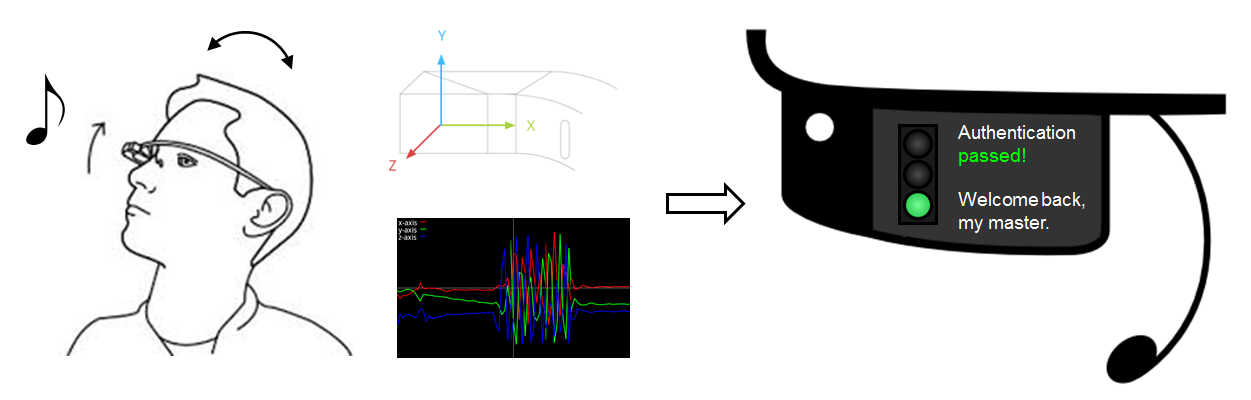
\includegraphics[width=.75\columnwidth]{../mobisys_paper/fig/headbanger-illustrate.png}
\caption{Illustration of Headbanger. The head-worn device authenticates the
right user based on signatures generated from head-movement patterns in
response to an audio snapshot played on the device.}
\label{fig:illustrate}
\end{figure}



\subsection{Overview of ~\systemname}

We refer to the proposed body-movement based authentication system tongue-in-cheek as~\systemname. We envision that~\systemname~will be used as an authentication interface on the wearable device, which will run upon device power-up, similar to the screen-lock in smartphones or the head-nod interface on Google Glass~\cite{googleglass}.  %~\systemname~keeps the real user's reference data and uses a classification approach to prove whether a user is the real user.

The authentication process has two parts: offline training and online authentication. In the offline training phase, the system collects the real user's body movement data and establish the features, which are referred to as \emph{reference} data. In the online authentication phase, we first ask the user to claim her ID from a list of user IDs (this can be done through simple gesture or voice). Next, we ask the user to pick a music track from a list of music tracks: if her pick does not match the claimed user's pick, then the authentication process exits immediately and returns FALSE. Otherwise,~\systemname~continues to go through the following steps:
\begin{itemize}
\vspace{-2pt}\item {\em Test sample collection}: In this step, we play the chosen music track for a few seconds (usually for up to 10 seconds), and ask the user to move along with the music. It is up to the user to decide which part of the body she will move(e.g., a combination of head, eye, arm, hand, leg, etc) and she will move. The advantages of using music as external stimuli are two-fold: (1) humans naturally respond to music beats by moving parts of their body, and (2) each person responds to music beats in different ways, and thus more user-specific information can be encoded in the movement pattern.

We record the raw sensor signals (e.g., from built-in accelerometer sensor or gyroscope sensor) during the music play period. We refer to the raw sensor data collected during a music track duration as a sample, e.g., an $ACC$ sample is the accelerometer data collected during the music period, and a $GYRO$ sample is the gyroscope data collected during the music period. After collecting the raw samples, we filter the samples to remove records of spurious motion so that the resulting sample will be much smoother and ready for subsequent processing.

\vspace{-2pt}\item {\em Classification}: In this step, we extract features from the filtered signal and run the classification algorithm against the reference data that was collected during the offline training phase. We will study a large set of features and classification algorithms and choose those that are suitable for wearable devices. If there is a plausible match, the user is accepted; otherwise, she is rejected.
\end{itemize}

Figure~\ref{fig:illustrate} illustrates the working of~\systemname. In this example, we try to authenticate Google glass users by monitoring their head movement patterns with music as external stimuli.


\subsection{Research Challenges}
Even though body movements have been used as biometric characteristics in other systems, it is completely unknown whether this method can be applied to wearable devices due to their unique constraints: (1) first, wearable devices are limited in battery/processing power and the types of sensors available to them, and (2) wearable devices should be able to deal with a much larger variety of body movements. Towards building a robust authentication system that solely runs on wearable devices, we strive to address two significant challenges in this project.

The first challenge is \emph{how we can establish body movement patterns as reliable biometric characteristics for authentication purposes.} In real life, it is common for us humans to recognize a person who is still far away by watching how she walks, i.e., her walking gait. To our brain, gait is unique, so are many other body movements. For example, by looking at how a person dances, we surely can recognize whether she is one of our friends.  However, 
whether the device we have, and/or the sensors available to the device, can capture, present, and quantify the uniqueness of these body movements, remains a challenge. The challenge is even more severe for seriously resource-constrained wearable devices and free-style natura movements. In this project, we will explore ways  to address this challenge. Towards this goal, we will find ways to pack as much as information in the sensor data, we will also try to authenticate users no matter they are stationary or walking, we will combine multiple movements that can be captured by a single wearable device, we will exploit multiple sensors to increase the authentication accuracy. For those users who desire a more secure authentication, we also exploit the fact that wearable devices can give out stimuli that only the wearer can feel to design body movement passwords which can greatly improve the authentication performance.

The second challenge is \emph{how we can minimize the resource consumption and processing delay of~\systemname~.} In order to achieve accurate classification results, it is often unavoidable to rely upon complex features and powerful classification algorithms, which will be very hard, if at all possible, to run on wearable devices. For this reason, wearable device authentication usually leverages a second device, which is much more powerful (e.g., smartphone). In this project, we take the viewpoint that authenticating users with two devices is inconvenient, and instead, we would like to implement the entire authentication process on the wearable device. To address this challenge, we propose to carefully choose the features and classifiers, and more importantly, we propose to pipeline the online authentication operations to significantly reduce the latency and power consumption. Finally, we also propose to dynamically adjust the sampling rate based upon the physical context information about the device.
